\documentclass[compress]{beamer}
\usepackage[ngerman]{babel}
\usepackage{graphicx}
\usepackage{subfiles}


\graphicspath{{resources/}}

% \setbeameroption{show notes}

\usetheme[noflama]{custom}

\title{Funktionale \break Programierung}
\subtitle{Nebenläufigkeit \& Parallelisierung}
\author{Jan-Philipp Willem}
\institute{
  Prof. Dr. Sandro Leuchter\\
  Fakultät für Informatik\\
  Hochschule Mannheim
}
\date{Seminar, WS2016}

\begin{document}

\begin{frame}[noframenumbering,plain]
  \frametitle{Was wird hier gezeigt?}
  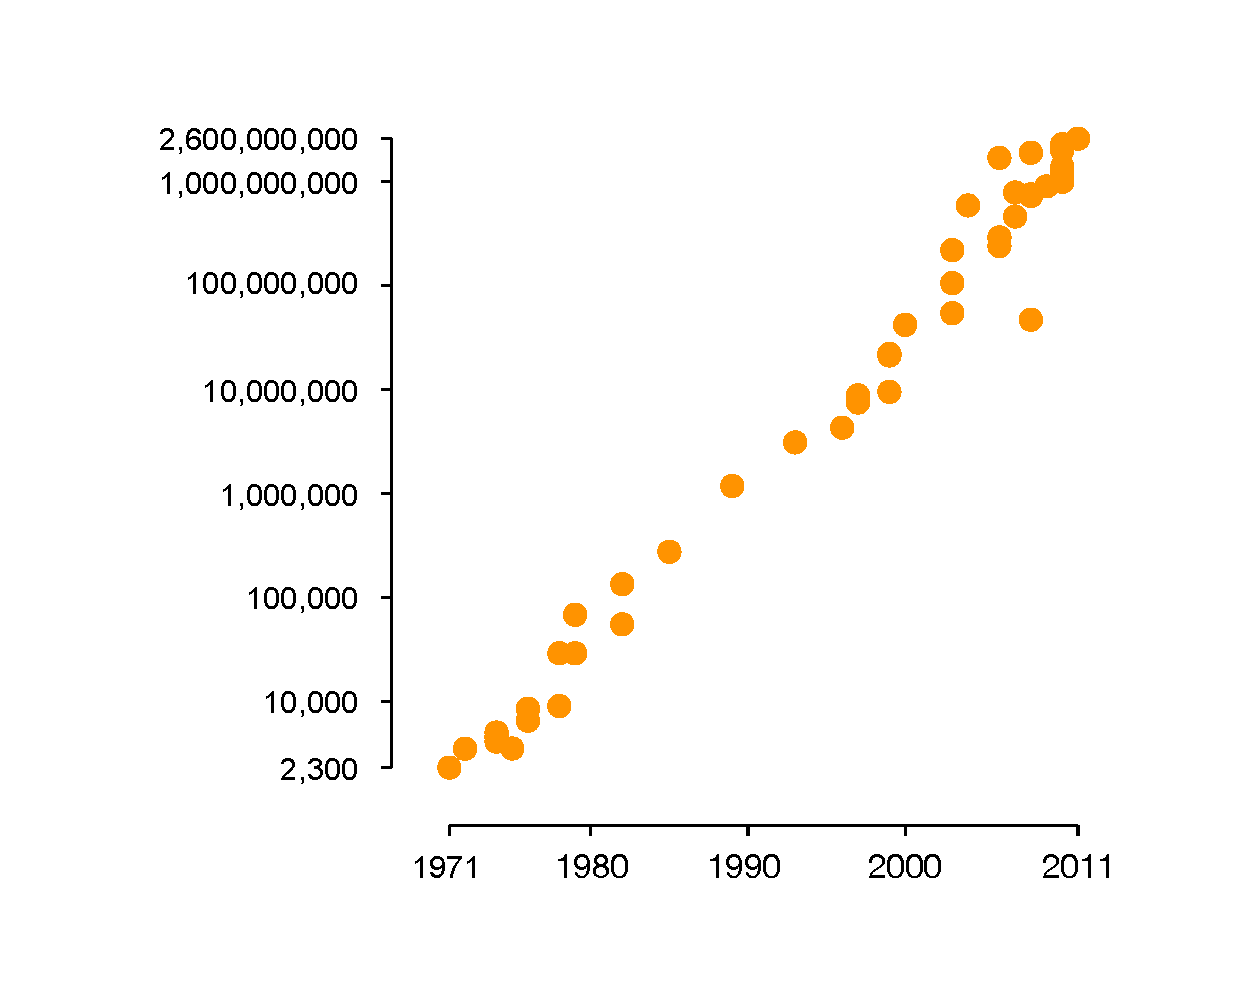
\includegraphics[width=0.9\textwidth]{moores_law.pdf}
\end{frame}
 
\begin{frame}[noframenumbering,plain]
  \frametitle{Transistor Counts 1971-2011 \& Moore's Law}
  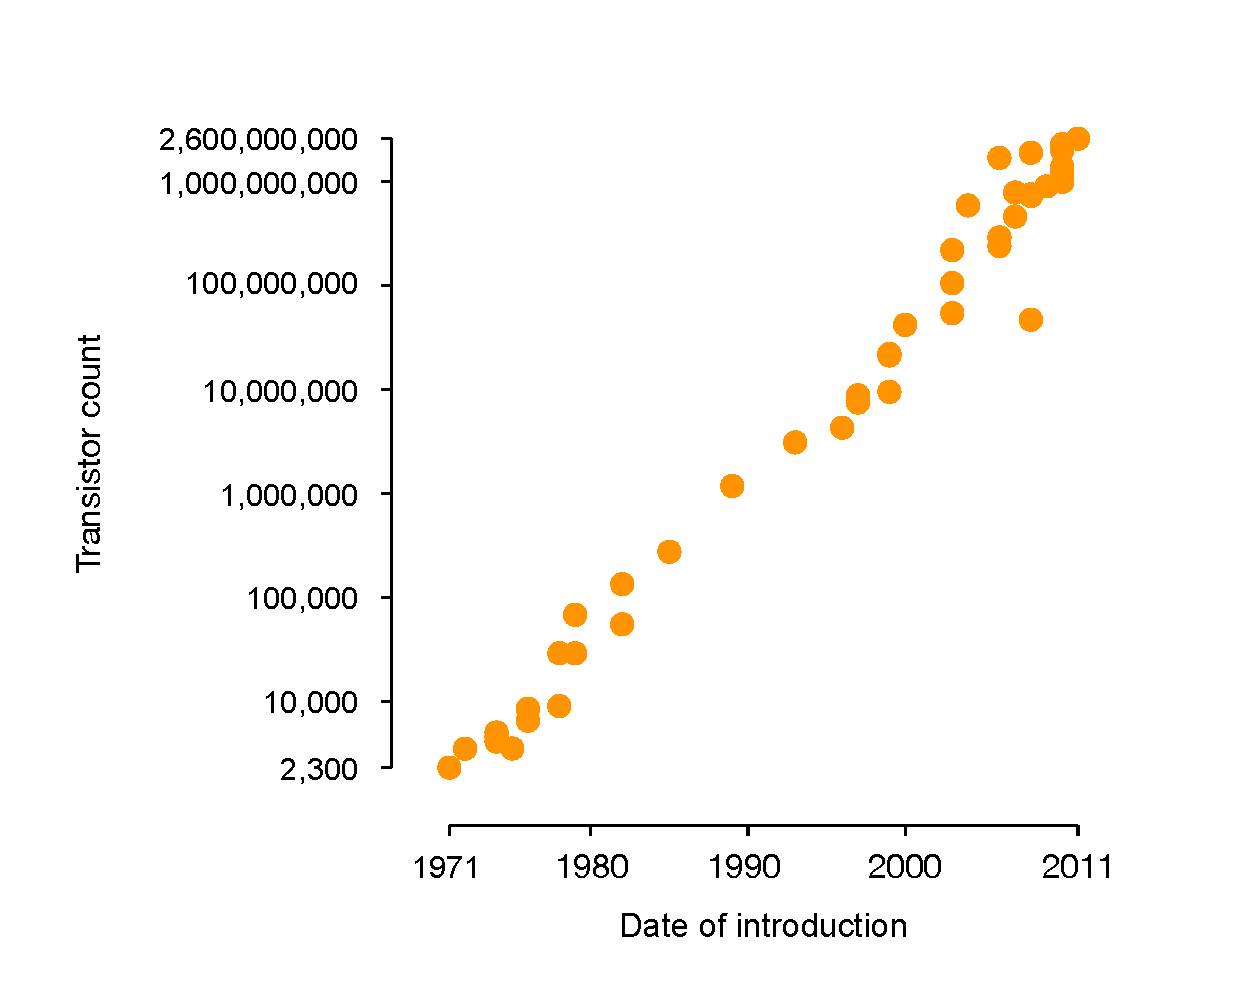
\includegraphics[width=0.9\textwidth]{moores_law_with-labels.pdf}
\end{frame}

\maketitle

\section*{Gliederung}
\begin{frame}[noframenumbering,plain]{Gliederung}
  \tableofcontents[hideallsubsections]
\end{frame}

\note[itemize]{
    \item The audience sees the slides, but you see your notes.
    \item Or, if your don't have notes, you can use mirror mode.
}


\section[Nebenläufigkeit oder Parallelisierung?]{Nebenläufigkeit / Parallelisierung}
  \begin{frame}{Parallel}
  \setcounter{framenumber}{1}
    \begin{columns}[c]
    \column{.5\textwidth}
      \begin{itemize}
        \item Synonyme: \texttt{nebeneinander, nebenläufig}
        \item Informatik:\\parallel ≠ nebenläufig !
        \item „schneller als sequenzielles Programm, durch \alert{gleichzeitiges} Ausführen von Anweisungen“
      \end{itemize}
    \column{.5\textwidth}
    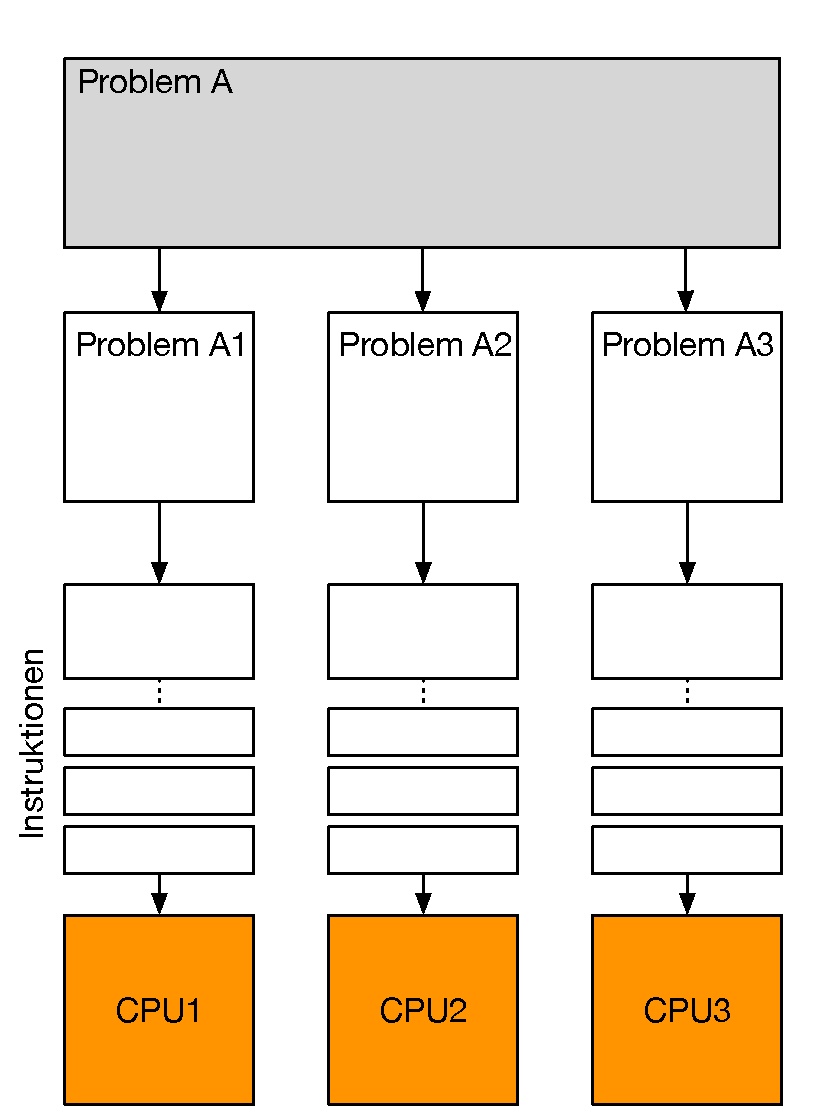
\includegraphics[width=\textwidth]{parallel.pdf}
    \end{columns}
  \end{frame}

  \note[itemize]{
      \item Im Vergleich zu sequenziellem Programm
      \item Aufteilen des Problems in Teilprobleme
      \item Teile können, müssen aber nicht zusammengehörend sein
  }

  \begin{frame}{Nebenläufig}
    \begin{itemize}
      \item Concurrent (engl.)
    \end{itemize}
  \end{frame}

  \begin{frame}{Rob Pike - 'Concurrency Is Not Parallelism'}
    \begin{itemize}
      \item „Concurrency is about dealing with lots of things at once.“
      \item „Parallelism is about doing lots of things at once.“
      \item „Concurrency is about structure, parallelism is about execution.“
    \end{itemize}
  \end{frame}

  \note[itemize]{
      \item Google, Go-Lang
      \item interessanter Talk auf Youtube
  }

\section{Threads / Locking}
  \begin{frame}{Was ist ein Thread?}
    \begin{itemize}
      \item Punkt 1
      \item Punkt 2
    \end{itemize}
  \end{frame}
  
  \begin{frame}{Häufige Bugs}
    \begin{columns}[c]
    \column{.5\textwidth}
      \textbf{Race-Condition}
      \begin{itemize}
        \item ++
        \item ++
      \end{itemize}
    \column{.5\textwidth}
      \textbf{Deadlock}
      \begin{itemize}
        \item --
        \item --
      \end{itemize}
    \end{columns}
  \end{frame}
  
  \begin{frame}{Fazit: Threads Programming}
    \begin{itemize}
      \item "State is Evil"
      \item Viele Sprachen besitzen threads als feature,
      \item wenige Sprachen helfen mit Tooling oder Abstraktion dem Programmierer selbst!
    \end{itemize}
  \end{frame}

\section{Functional Paradigm 101}
  \begin{frame}{Functional Paradigm 101}
    \begin{itemize}
      \item reine Funktionale Sprachen
      \item imutable // mutable
      \item no side-effects
      \item deterministic
      \item data-in <-> data-out
      \item functions as first-class citizens
      \item lamdas
    \end{itemize}
  \end{frame}

\section{Elixir}
  \begin{frame}{Elixir}
    \begin{itemize}
      \item moderne Variante von Erlang (1987, Ericsson)
      \item Beam-VM
      \item Fault-Taulerant
      \item „Let it crash“
      \item Supervision-Trees
      \item Shared \& Distributed Memory
      \item Open Telecom Platform (OTP)
    \end{itemize}
  \end{frame}

  \begin{frame}{OTP / Actor-Model}
    \begin{columns}[c]
    \column{.5\textwidth}
    \begin{itemize}
      \item Punkt 1
      \item Alternativen:
        \begin{itemize}
          \item Akka (Java/Scala)
          \item Akka.NET
          \item Pykka (Python)
          \item CAF (C++)
          \item Celluloid (Ruby)
        \end{itemize}
    \end{itemize}
    \column{.5\textwidth}
      Img-Exp
    \end{columns}
  \end{frame}
  
  \begin{frame}{List-Processing in Elixir: map}
  \end{frame}

  \begin{frame}{List-Processing in Elixir: reduce}
  \end{frame}

  \begin{frame}{List-Processing in Elixir: filter}
  \end{frame}

  \begin{frame}{Elixir-Streams}
  \end{frame}

\section{Fazit}
  \begin{frame}{Fazit: Functional Programming}
    \begin{columns}[c]
    \column{.5\textwidth}
      \textbf{Vorteile}
      \begin{itemize}
        \item Punkt 1
        \item Punkt 2
      \end{itemize}
    \column{.5\textwidth}
      \textbf{Nachteile}
      \begin{itemize}
        \item Punkt 1
        \item Punkt 2
      \end{itemize}
    \end{columns}
  \end{frame}
  
  \begin{frame}{Functional Style in Imperative Languages}
  \end{frame}
\end{document}
